\documentclass{exercise}

\institute{Applied and Computational Mathematics}
\title{Selbstrechenübung 5}
\author{Joshua Feld, 406718}
\course{Mathematische Grundlagen IV}
\professor{Torrilhon \& Berkels}
\semester{Sommersemester 2022}
\program{CES (Bachelor)}

\begin{document}
    \maketitle


    \section*{Aufgabe 1}
    
    \begin{problem}
        Gegeben sei das glatt berandete Gebiet \(\Omega\) wie in der folgenden Abbildung mit den Rändern \(\Gamma_1\) und \(\Gamma_2\).
        Gesucht wird eine Funktion \(u \in C^2\parentheses*{\Omega}\) mit
        \begin{align*}
            -\Delta u\parentheses*{x} &= 0, \quad x \in \Omega,\\
            u\parentheses*{x} &= 1, \quad x \in \Gamma_1,\\
            u\parentheses*{x} &= 0, \quad x \in \Gamma_2.
        \end{align*}
        \begin{center}
            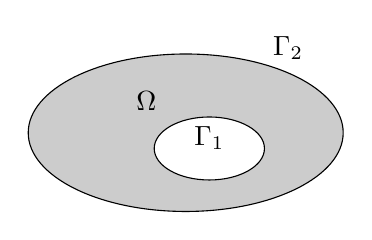
\begin{tikzpicture}
                \draw[fill=white!80!black] (0,0) ellipse (2cm and 1cm);
                \draw[fill=white] (.3,-.2) ellipse (.7cm and .4cm);
                \node[anchor=north] at (.3,.2) {\(\Gamma_1\)};
                \node[anchor=south] at (1.3,.8) {\(\Gamma_2\)};
                \node at (-.5,.4) {\(\Omega\)};
            \end{tikzpicture}
        \end{center}
        \begin{enumerate}
            \item Zeigen Sie, dass \(u\) auf \(\Omega\) beschränkt ist, und geben Sie eine untere und eine obere Schranke an.
            \item Zeigen Sie
            \begin{align*}
                \partial_n u &= \nabla u \cdot n \ge 0\text{ auf }\Gamma_1,\\
                \partial_n u &= \nabla u \cdot n \le 0\text{ auf }\Gamma_2,
            \end{align*}
            wobei \(n\) der äußere Normalvektor auf \(\Gamma_1\) bzw. \(\Gamma_2\) ist.

            \emph{Hinweis: \(\partial_n u = \lim_{h \to 0}\frac{1}{h}\parentheses*{u\parentheses*{x} - u\parentheses*{x - hn}}\)}
        \end{enumerate}
    \end{problem}
    
    \subsection*{Lösung}


    \section*{Aufgabe 2}
    
    \begin{problem}
        Betrachten Sie das Randwertproblem für Konstanten \(c_1, c_2 \in \R\)
        \begin{align*}
            -u''\parentheses*{x} - c_1 u\parentheses*{x} &= 0, \quad x \in \parentheses*{0, 1},\\
            u\parentheses*{0} &= 0,\\
            u\parentheses*{1} &= c_2.
        \end{align*}
        \begin{enumerate}
            \item Bestimmen Sie das Gleichungssystem
            \[
                Au_h = b,
            \]
            mit \(A \in \R^{n \times n}\) und \(b \in \R^n\), das sich aus einer Diskretisierung der Differentialgleichung mit zentralen finiten Differenzen zweiter Ordnung für \(u''\) mit der Schrittweiter \(h = \frac{1}{n + 1}\) ergibt.
            \item Zeigen Sie, dass die Matrix \(A\) die Eigenwerte
            \[
                \lambda_k = \frac{4}{h^2}\sin^2\parentheses*{\frac{k\pi h}{2}} - c_1, \quad k = 1, \ldots, n
            \]
            und die zugehörigen normierten Eigenvektoren
            \[
                v_k = \sqrt{2h}\parentheses*{\sin\parentheses*{k\pi h}, \sin\parentheses*{2k\pi h}, \ldots, \sin\parentheses*{nk\pi h}}^T
            \]
            besitzt.
            \item Lösen Sie das Gleichungssystem für \(c_1 := \pi^2\) mit dem Ansatz
            \[
                u_h = \sum_{i = 1}^n \alpha_i v_i
            \]
            und bestimmen Sie die Koeffizienten \(\alpha_i\) durch geeignete Skalarprodukte.
            Prüfen Sie, ob der so berechnete Ausdruck für \(\alpha_i\) wohldefiniert ist.

            \emph{Hinweis: Für \(x \in \left(0, 1\right]\) gilt \(\arcsin\parentheses*{x} < \frac{\pi}{2}x\).}
            \item Zeigen Sie für \(c_1 := \pi^2\) und \(c_2 > 0\), dass die erste Komponente \(u_1\) der Lösung \(u_h\) für \(h \to 0\) gegen \(-\infty\) divergiert.

            \emph{Hinweis: Verwenden Sie die Taylorentwicklungen
            \begin{align*}
                \sin^2\parentheses*{ah} &= a^2 h^2 - \frac{1}{3}a^4 h^4 + \mathcal{O}\parentheses*{h^6},\\
                \sin\parentheses*{ah}\sin\parentheses*{a\parentheses*{1 - h}} &= ah\sin\parentheses*{a} - a^2 h^2 \cos\parentheses*{a} + \mathcal{O}\parentheses*{h^3}.
            \end{align*}}
            \item Was lässt sich über die analytische Lösung des Randwertproblems für \(c_1 := \pi^2\) sagen?
        \end{enumerate}
    \end{problem}
    
    \subsection*{Lösung}
\end{document}
